\chapter{Programmentwurf und -implementierung}
\label{chap:entwurf}

In diesem Kapitel m"ochte der Autor die Entwicklung des Gesamtprogramms er"ortern.
Es wird ein "Uberblick "uber das umfassende Konzept des internen Aufbaus gegeben um anschlie\ss end auf die konkrete Umsetzung der einzelnen Bestandteile einzugehen.
Demzufolge sind die kommenden Abschnitte nach den Programmkomponenten gegliedert.
In jedem einzelnen Abschnitt wird auf drei Punkte eingegangen:
\begin{itemize}
	\item Grundlegende Idee und Designkonzept
	\item Implementierungsdetails
	\item Tests zur Verifikation der einzelnen Komponente
\end{itemize}
Es sei darauf hingewiesen, dass die eigentlichen Entwicklung und Implementierung nicht Komponentenweise, sondern nach entsprechenden Funktionalit"aten statt findet.
Das Einbinden einer bestimmten Funktionalit"at betrifft oft mehrere Komponenten und ihr Zusammenspiel, wodurch der Ausbau der einzelnen Bestandteile parallel geschieht.
Die Gliederung dieses Kapitels nach den Programmteilen dient jedeglich der "Ubersichtlichkeit.

\section{"Uberblick "uber das Gesamtprogramm}

Das Programm ist in verschiedene Pakete geteilt (vgl. \picref{paket_ubersicht}).
Die Teilung der einzelnen Komponenten erfolgt haupts"achlich nach ihrer Funktionalit"at.
In dem Hauptpaket \code{gst} befinden sich nur zwei Klassen:
Die Klasse \class{Main}, die die statische Methode f"ur den Programmstart und globale Initialisierungsroutinen beinhaltet, und die die Klasse \class{Settings}.
Mit \class{Settings} werden Variablen bereit gehalten die f"ur das Programm konstant sind, aber auf Wunsch auch ver"andert werden k"onnen.
Die Idee hinter dieser Implementierung ist die, dass "Anderungen die das allgemeine Verhalten und Aussehen des Programms beeinflussen m"oglichst zentral verwaltet werden und sich diese Optionen nicht "uber den gesamten Quellcode verteilt sind.
Es soll damit eine einfacherer Wartbarkeit der Umsetzung erreicht werden.

Ein gro{\ss}es Teilpaket ist \code{data}.
In diesem befinden sich Klassen die direkt mit dem Zugriff auf Daten, den Datensatz und die Ver"anderung von Daten besch"aftigen.
Diese Paket ist im Detail im \secref{data} beschrieben.
Das zweite Kernpaket des Programms ist \code{ui} und beinhaltet Klassen die direkt mit der \ac{GUI} der Benutzerinteraktion in Ber"uhrung kommen.
Das \code{ui}-Paket hat noch zwei Unterpakete:
\code{dialog} enth"alt Klassen die das Aussehen und die Interaktion mit Dialogfenstern implementieren.
Das Unterpaket \code{layout} umfasst Klassen die ben"otigt werden um die Anordnung der einzelnen grafischen Elemente der \ac{GUI} zu organisieren.
Das \code{ui}-Paket selbst und seine Klassen sind im \secref{gui} beschrieben.
Ein drittes umfangreiches Paket ist das \code{signalprocessing}-Paket und enth"alt Quellcode der den Grundbaustein f"ur die Signalverarbeitung.
Der Aufbau und die Funktionsweise des dritten Pakets ist im \secref{signalprocessing} dargelegt.

Letztendlich existieren im \code{test}-Paket noch zwei Klassen, die haupts"achlich die Entwicklung des Programms selbst unterst"utzen.
Die Klasse \class{Debug} bietet eine Methode zum ausgeben von Informationen auf der Konsole die f"ur den Entwickler bestimmt sind.
"Uber ein Feld von booleschen Variablen k"onnen f"ur jede Klasse des Programms die Debugmeldungen ein- und ausgeschaltet werden.
Somit ist es nicht notwendig den Quelltext der einzelnen Klassen zu ver"andern nur um die oben genannten Meldungen abzuschalten.
Zus"atzlich zur Klasse \class{Debug} existiert im \code{test}-Paket noch die Klasse \class{DataTest}.
In ihr sind Methoden implementiert, die die Funktionalit"at einzelner Klassen und die Interaktion der Objekte miteinander "uberpr"uft.
Die \class{DataTest} Klasse hat, ebenso wie \class{Debug}, den Zweck w"ahrend der Entwicklung Fehler in der Implementierung aufzudecken und dienen haups"achlich dem Informationsgewinn des Entwicklers.
Aus diesem Grund wird das \code{test}-Paket in dieser Arbeit auch nicht n"aher erl"autert.

\begin{figure}[htb]
\centering
\includegraphics[angle=-90, width=0.9\textwidth]{bilder/programm_overview.pdf}
\caption[\acs{uml}-Paket-"Ubersicht der umgesetzten Software]{\ac{uml}-Paket-"Ubersicht der umgesetzten Software, nur wesentliche Klassen sind dargestellt}
\label{pic:paket_ubersicht}
\end{figure}

%\begin{table}[hbt]
%\centering
%\caption[Paket- und Klassen"ubersicht]{Paket- und Klassen"ubersicht: Paketnamen sind in \texttt{True-Type} und Klassennamen in \textsf{serifenloser} Schriftart geschrieben}
%\label{tab:klassenubersicht}
%\textsf{
%	\begin{tabular}{|llll|}
%		\hline
%		\texttt{gst} & Main &&\\ 
%		    		 & Settings &&\\\hline
%		\texttt{gst.}& \texttt{data} & AnnotationController &\\
%					 &				 & AnnotationList &\\
%					 &				 & AnnotationManager &\\
%					 &				 & DataController &\\
%					 &				 & SignalController &\\
%					 &				 & UnisensDataset &\\
%					 &				 & ValueController &\\\hline
%		\texttt{gst.}& \texttt{test} & DataTest &\\
%					 &				 & Debug &\\\hline
%		\texttt{gst.}& \texttt{ui}	 & AnnotationSelectionDialog &\\
%					 &				 & DataSelectionDialog &\\
%					 &				 & MainWindow &\\
%					 &				 & Menus &\\
%					 &				 & NamedMouseAdapter &\\
%					 &				 & Sidebar &\\
%					 &				 & SignalOverview &\\
%					 &				 & SignalPanel &\\
%					 &				 & SignalView &\\
%					 &				 & SignalViewFactory &\\
%					 &				 & StatusBar &\\
%					 &				 & Toolbar &\\\hline
%		\texttt{gst.}& \texttt{ui.}	 & \texttt{dialog} & DatasetSelectionDialog\\
%					 &				 &				   & EditEventDialog \\
%					 &				 &				   & EnterFileNameDialog \\\hline
%		\texttt{gst.}& \texttt{ui.}	 & \texttt{layout} & ComponentArrangement \\
%					 &				 &				   & MultiSplit\\
%					 &				 &				   & SignalPanelLayoutManager\\
%					 &				 &				   & VerticalLayoutManager\\\hline
%\end{tabular}
%}
%\end{table}

%-- theoretische beschreibung des gesamtkonzeptes
%-- komplette auflisten der subkomponenten in \tabref{klassenubersicht}
%-- graphische "Ubersicht der Bestandteile siehe \picref{paket_ubersicht}


\section{Datenbehandlung}

Aufgrund der Vielfalt der genutzten Datenformate zur Speicherung von Biosignalen und der Nichtexistenz eines einheitlichen Standards \cite{Schlogl2009, Varri2001, Wang2010} muss ein Format gesucht werden, dass zur Behandlung von Datens"atzen im Rahmen dieser Arbeit geeignet ist.
Die Wahl des Datensatzformates st"utzt sich auf die vergleichende Untersuchung \cite{Schlogl2009} von Dr. Alois Schl"ogl der Technischen Universit"at Graz.
Das Unisens-Format besitzt eine Referenzimplementierung mit Programmierschnittstellen sowohl f"ur Matlab als auch f"ur Java und bietet f"ur diese Arbeit optimale Anwendungsvoraussetzungen.
Die Organisation "uber eine menschlich les- und editierbare Headerdatei ist gerade in der Entwicklung interessant.
Es kann ein Datensatz einfach und ohne Bearbeitungstools ver"andert und an die Bed"urfnisse angepasst werden.
Einer der Kritikpunkte nach \cite{Schlogl2009} ist, dass das Format aus mehreren Dateien besteht.
Da die Behandlung von Dateien und Verzeichnissen mit der aktuellen Software kaum noch Unterschiede f"ur den Anwender darstellt, ist nach Meinung des Autors dieser Punkt nicht von hoher Priorit"at.
Es bietet sogar die M"oglichkeit Daten direkt von Sensoren (bei bekannten technischen Parametern wie z.B. Abtastrate und -aufl"osung) direkt in einen Datensatz integriert werden k"onnen.
Zus"atzlich bietet das Format durch seine Definition eine gute Erweiterbarkeit.
Es kann somit an die neue Gegebenheiten und Voraussetzungen angepasst und optimiert werden.

%	-- menschlich editierbar (xml header)
%	-- verzeichnis vs eine datei ist vernachl"assigbar
%	-- reine sensordaten importierbar
%	-- implementierung vorhanden
%	-- f"ur matlab und java

\subsection{Unisens}

Das vom Forschungszentrum Informatik und Institut f"ur Technik der Informationsverarbeitung der Universit"at Karlsruhe entwickelte Datenformat Unisens dient der Speicherung und der Dokumentation von Sensordaten.
Unisens ist konzipiert, Daten verschiedener Sensoren innerhalb eines Datensatzes zu speichern.
Ein Datensatz ist im Dateisystem durch ein eigenes Verzeichnis und eine Headerdatei \verb|unisens.xml| hinterlegt.
In der Headerdatei werden alle Informationen "uber die Bestandteile des Datensatzes, deren Formatierung und ihre semantischen Zusammenh"ange gespeichert.
Messwerte eines Sensors werden "ublicherweise in einer Datendatei innerhalb des Datensatzverzeichnisses abgespeichert.
Eine solche Datendatei wird als \emph{Entry} in dem Datensatz bezeichnet.
Alle Metainformationen zu den Sensordaten werden in der Headerdatei abgspeichert, so dass die Datendateien selbst immer nur die reinen Messdaten enthalten.
Als m"ogliche Sensordaten werden sowohl kontinuierlich abgetastete Signale als auch ereignisorientierte Daten unterst"utzt.
Unisens unterscheidet zwischen vier Arten von Daten:
\begin{description}
	\item[Signale \emph{(Signal)}] \hfill \\
		Signale sind "aquidistant abgetastete, numerische Messdaten.
		Sie zeichnen sich durch eine beliebige aber konstante Abtastrate und Abtastaufl"osung aus.
		Zudem k"onnen Signale aus mehreren Kan"alen bestehen, die alle in ein und derselben Datei abgespeichert werden.
		Alle Kan"ale desselben Signals haben auch dieselbe Abtastrate und -aufl"osung.
	\item[Ereignisse \emph{(Event)}] \hfill \\
		Ereignisse sind diskrete Zeitpunkte die mit einer textlichen Beschreibung versehen sind. (z.B. Triggersignale)
		Sie zeichnen sich durch einen Zeitstempel und einer kurzen Beschreibung aus.
		Optional k"onnen noch Kommentare zu einem Ereignis hinzugef"ugt werden.
	\item[Einzelwerte \emph{(Value)}] \hfill \\
		Einzelwerte sind eine Kombination der beiden oben genannten Datenarten.
		Sie beinhalten numerische Werte die zu bestimmten Zeitpunkten aufgenommen wurden.
		Mit Einzelwerten ist es m"oglich Daten zu speichern, die nicht in festen Zeitintervallen gemessen werden.
	\item[Propriet"are Daten \emph{(Custom data)}] \hfill \\
		Mit dieser Art k"onnen anwendungsspezifisch Daten gespeichert werden, die durch die drei oben genannten Arten nicht erfasst werden k"onnen.
		So k"onnen beispielsweise schematische Darstellungen des Messaufbaus als Bilddateien oder Patienteakten in Form von Textdateien dem Datensatz hinzugef"ugt werden.
\end{description}
Eine detailiertere Beschreibung des Formates kann der offiziellen Dokumentation \cite{Ottenbacher2010} entnommen werden.

\subsubsection{Details der Referenzimplementierung}

In diesem Abschnitt wird kurz auf einige Details der Umsetzung des Unisens-Formates eingegangen.
Das Unisens-Paket ist in Java implementiert und wird unter der \emph{\ac{lgpl}} zur Verf"ugung gestellt.
Die bereit gestellte Bibliothek ist auf zwei Einzeldateien aufgeteilt: \verb|org.unisens.jar| und \verb|org.unisens.ri.jar|.
Bei der ersten Datei handelt es sich um die Definiton des Unisensformates und seiner Bestandteile als Javalassenstruktur.
Diese Definition erfolgt haupts"achlich als \emph{Interface}klassen und legt die Schnittstellen zwischen den einzelnen Bestandteilen fest.
Eine "Ubersicht der Klassenstruktur und der von au\ss en ersichtlichen Attribute ist in \picref{unisens_interface} auf Seite \pageref{pic:unisens_interface} dargestellt.
\begin{sidewaysfigure}%[h]
\centering
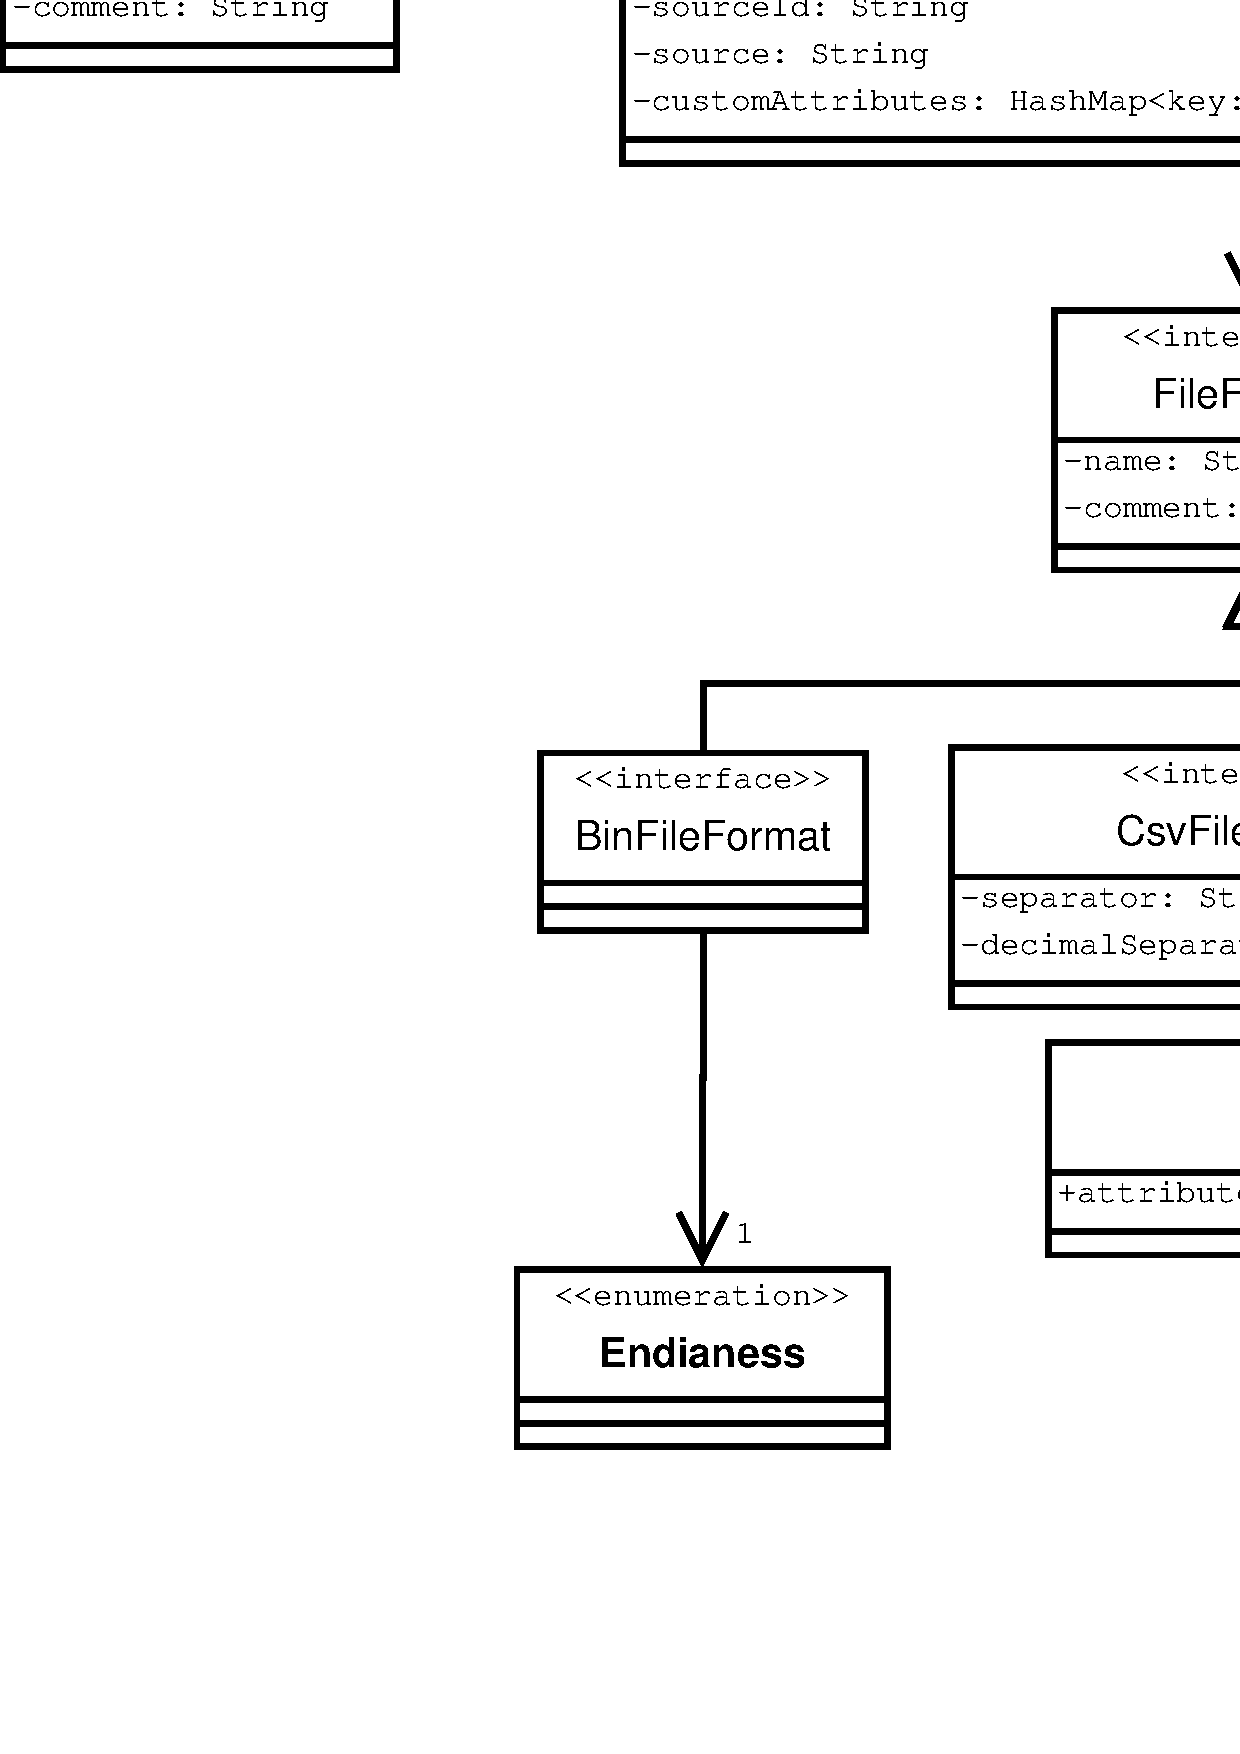
\includegraphics[angle=-90, width=0.9\textwidth]{bilder/unisens_interface_.pdf}
\caption{Klassen"ubersicht der von Unisens definierten Schnittstellen}
\label{pic:unisens_interface}
\end{sidewaysfigure}
Die vom Unisensformat unterst"utzten Signalarten sind auch in der Klassenstruktur in \tabref{unisens_signalklassen} erkennbar.
\begin{table}[h]
\centering
\begin{tabular}{|c|c|}
	\hline Signale & \verb|SignalEntry| \\
	\hline Ereignisse & \verb|EventEntry| \\
	\hline Einzelwerte & \verb|ValuesEntry| \\
	\hline Propriet"are Daten & \verb|CustomEntry| \\
	\hline
\end{tabular}
\caption{Signalarten und ihre repr"asentierenden Klassen}
\label{tab:unisens_signalklassen}
\end{table}

Aufgrund der Ableitung der Klassen \verb|EventEntry| und \verb|ValuesEntry| von \verb|TimedEntry| ist ersichtlich, dass die Zeitpunkte von Ereignisdaten und Einzelwertdaten "uber eine virtuelle Abtastrate bestimmt werden.
Der Zeitpunkt eines jeden \emph{Event}- oder \emph{Value}-Eintrags ist als ganzzahlige Samplenummer dieser Abtastrate gespeichert.
Die Zeit eines Ereignisses, relativ zum Messbeginn, errechnet sich somit $Zeitpunkt = {Samplenummer \over Abtastrate}$.
M"ochte man die M"oglichkeit Ereignisse f"ur jeden beliebigen Datenpunkt eines Datensatzes zuordnen zu k"onnen, dann muss die virtuelle Abtastrate als das kleinste gemeinsame Vielfache aller vorhandenen Abtastraten gew"ahlt werden.

Die Schnittstellendefinition des Unisensformats stellt nur Methoden zum Lesen und Anh"angen von Datenpunkten an den Datensatz bereit.
Somit wird ein Einf"ugen, L"oschen oder Ver"andern von Datenpunkten innerhalb eines Dateneintrags nicht unterst"utzt.
Sollen diese Funktionen vorhanden sein, so muss diese Funktionalit"at selbst implementiert werden.

Die eigentliche Umsetzung der Funktionalit"at ist in der zweiten Datei abgespeichert.
Im Folgenden soll sich der Begriff Referenzimplementierung auf diese funktionelle Umsetzung beziehen.
Die Klassen der Referenzimplementierung bestehen aus den Klassennamen der Schnittstellendefinition und dem Suffix "`Impl"' (z.B. Objekte die den Datensatz darstellen haben die Klasse \verb|UnisensImpl|).
Wenn man schon vorhandene Unisensdatens"atze benutzen m"ochte reicht es aus, die Schnittstellendefinition zu kennen und zu nutzen.
Sollen hingegen konkret Objekte erstellt werden, muss auf die Referenzimplementierung zur"uckgegriffen werden.

Durch einen Fehler in der Referenzimplementierung kann es vorkommen, dass beim Laden eines vorhandenen Unisensdatensatzes in dem Gruppen definiert sind eine \verb|NullPointerException| auftritt.
Insbesondere tritt dieser Fehler auf, wenn innerhalb der Headerdatei der Gruppeneintrag nicht hinter den Dateneintr"agen steht.

\subsection{Programminterne Datenstruktur}

\begin{figure}[htb]
\centering
\includegraphics[angle=-90, width=\textwidth]{bilder/package_data_ubersicht.pdf}
\caption[\acs{uml}-Diagramm des \texttt{data}-Paketes]{\ac{uml}-Diagramm des \texttt{data}-Paketes inklusive der bereitgestellten Schnittstellen}
\label{pic:data_package}
\end{figure}

Das Paket \verb|gst.data| ist die Schnittstelle der Programms zu dem gew"ahlten Datensatzformat Unisens.
Eine "Ubersicht des Paketes ist im \ac{uml}-Diagramm in \picref{data_package} dargestellt.
Dieses Paket erf"ullt zwei wesentliche Aufgaben:
\begin{itemize}
	\item Vereinheitlichung der Behandlung der unterschiedlichen Datenarten
	\item Abkapselung anderer Programmteile vom Datensatzformat
\end{itemize}

Die Vereinheitlichung ist notwendig, da Unisens die Daten in drei Arten gliedert: Signale, Werte und Ereignisse.
F"ur die Bearbeitung und Darstellung ist aber die Unterscheidung von Signalen und Werten nicht notwendig.
In beiden F"allen handelt es sich um numerische Werte die zu einem bestimmten Zeitpunkt aufgenommen wurden.
Somit sollen diese auch vom Programm gleichartig behandelt werden.
Daher erhalten alle Datenarten die abstrakte Klasse \verb|DataController| als Fassade.
Die jeweilge konkrete Implementierung ist in den drei abgeleiteten Klassen \verb|Signal-|, \verb|Value-| und \verb|AnnotationController| realisiert.
Neben der Vereinheitlichung der Schnittstelle zum Datensatz werden auch die Zugriffe auf die Daten vereinfacht.
Es werden notwendige Ausnahmebehandlungen (\emph{Exceptions}) durch die Klassen des \verb|data|-Paketes abgefangen und behandelt.
Darunter f"allt unter anderem die Behandlung von Fehlern, wenn Daten aufgrund von fehlenden Zugriffsrechten nicht gelesen oder geschrieben werden k"onnen.
Somit ist der Zugriff auf die konkreten Daten des Datensatzes sowohl vereinheitlicht als auch vereinfacht.

Weiterhin wird mit dem \verb|data|-Paket erreicht, dass die restlichen Komponenten des Programms nicht direkt auf das Datensatzformat zugreifen.
Sie sind damit von dem gew"hlten Format abgekapselt und ein Austausch des Formates erfordert nur die Anpassung des \verb|data|-Paketes.
Der gesamte Datensatz ist durch die Wrapper-Klasse \verb|UnisensDataset| im Programm repr"asentiert.
Zugriff auf den Datensatz erfolgt nur "uber die von der Klasse bereitgestellte Schnittstelle.
Weiterhin wird der ver"anderde Zugriff auf Annotationen durch die Klasse \verb|AnnotationManager| realisiert und die Behandlung von Annotationen selbst "uber die Klasse \verb|AnnotationList| abgewickelt.
Die zwei zu letzt genannten Klassen kapseln die von Unisens bereitgestellten Klassen (\verb|Event| und \verb|EventList|) von den anderen Programmteilen ab.

Neben den zwei oben genannten Aspekten wird auch der Zugriff auf die Daten selbst durch das Paket ver"andert.
Unisens arbeitet durchgehend mit Samplenummern bei der Indizierung der einzelnen Datenpunkte.
Die durch das Paket bereitgestellte Schnittstelle wandelt diese Art des Zugriffs auf eine zeitbasierte Art um.
Das bedeutet, anstatt Daten "uber die Angabe von Samplenummern zu erhalten, bietet die Schnittstelle die M"oglichkeit Daten aus einem bestimmten Zeitraum zu erhalten.
Die notwendige Umrechnung zwischen Samplenummern und Abtastraten auf entsprechende Zeitpunkte wird im \verb|data|-Paket ausgef"uhrt.
Dadurch wird die Existenz verschiedener Abtastraten der unterschiedlichen Signale vor dem restlichen Programm verborgen.

\subsubsection{Repr"asentation des Datensatzes durch die Klassen \texttt{UnisensDataset} und \texttt{DataController}}

Die Klasse \verb|UnsiensDataset| stellt die Schnittstelle des Programms zu den Datens"atzen dar.
F"ur jeden geladenen Datensatz wird im Programm ein Objekt der Klasse \verb|UnisensDataset| erzeugt.
Diese Objekte bieteten die erforderlichen Funktionen um auf die Eigenschaften des Datensatzes, die Eigenschaften der Dateneintr"age und die Daten der Eintr"ge selbst zuzugreifen.
Beim Laden eines Datensatzes wird f"ur jeden Dateneintrag ein Instanz eines \verb|DataController|s erzeugt und in einer Liste \verb|ctrlList| im \verb|UnisensDataset|-Objekt gespeichert.
Je nach Datenart des Eintrags wird zur Laufzeit dynamisch ein Objekt der Klassen \verb|Signal-|, \verb|Value-| oder \verb|AnnotationController| erzeugt.
Genauer wird sogar f"ur jeden Kanal ein eigener \verb|DataController| angelegt.
Jede Komponente des Programms die auf einen Dateneintrag zugreifen m"ochte, erh"alt vom \verb|UnisensDataset| den entsprechenden Controller.
Es wird sichergestellt, dass zu jedem Zeitpunkt jedem Dateneintrag genau ein Controllerobjekt zugeordnet ist und keine Duplizierung auftreten kann.
Durch spezielle Funktionen \verb|AddNewSignal()|, \verb|AddNewValue()| und \verb|AddNewAnnotation()| k"onnen einem Datensatz zus"atzliche Dateneintr"age hinzugef"ugt werden.
Die entsprechenden \verb|DataController| werden dann in die Liste \verb|ctrlList| aufgenommen und es kann durch diese anschlie\ss end auf die Daten zugegriffen werden.
Der gesamte Datensatz wird bei einem Aufruf der \verb|save()|-Funktion des Datensatzes abgespeichert werden, weil die Speicherfunktion f"ur alle \verb|DataController|-Objekte in \verb|crtlList| rekursiv ausgef"uhrt werden k"onnen.

\subsubsection{Das Singleton-Konzept und \texttt{DatasetList}}

Die geladenen Datens"atze sollen im Programm in einer Liste zusammengefasst werden.
Diese Liste soll im gesamten Programm zug"anglich sein.
Es muss aber sichergestellt werden, dass ein und derselbe Datensatz nicht mehrfach geladen wird und somit mehrere Instanzen der Klasse \class{UnisensDataset} f"ur diesen angelegt werden.
Diese Aufgabe wird durch die Klasse \class{DatasetList} "ubernommen, die als Singleton-Klasse implementiert ist (siehe \picref{datasetlist}).
\begin{figure}[htb]
\centering
\includegraphics[angle=-90, width=0.8\textwidth]{bilder/singleton_datasetlist.pdf}
\caption[Klasse \texttt{DatasetList} und das Singleton-Konzept]{Die Klasse \texttt{DatasetList} und das Singleton-Konzept. Aus Gr"unden der "Ubersicht sind nicht alle Funktionen aufgelistet (durch \code{...()} markiert).}
\label{pic:datasetlist}
\end{figure}

Das Entwurfsmuster des Singletons (\cite{Gamma1995} Seite 127 bis 134) wird angewendet, wenn f"ur eine Klasse nur genau ein Objekt instanziert werden soll.
Es stellt zus"atzlich sicher, dass die geschaffene Instanz global im Programm erreichbar ist.
Damit die Einzigartigkeit des Objektes dieser Klasse garantiert ist, ist der Konstruktor der Klasse als \code{private} deklariert.
Somit kann keine neue Objektinstanz au{\ss}erhalb der Klasse \class{DatasetList} erzeugt werden.
Die Instanz selbst wird in der Klassenvariable \code{instance} gespeichert.
Klassenvariablen werden in der Klasse selbst gespeichert und nicht f"ur die einzelnen Objekte dieser Klasse angelegt.
Von au{\ss}en kann auf das konkrete Objekt "uber die "offentliche (\code{public}) Klassenfunktion \code{getInstance()} zugegriffen werden.
Klassenfunktionen sind wie Klassenvariablen f"ur die Klassen definiert, aber nicht f"ur die Objekte selbst.
Durch diese Singletonimplementierung ist sichergestellt, dass
\begin{itemize}
	\item die Objektinstanz \code{instance} der Klasse \class{DatasetList} innerhalb des Programms einzigartig ist und
	\item diese Instanz global im Programm "uber die Funktion \code{DatasetList.getInstance()} erh"altlich ist.
\end{itemize}

Die Objekte der \class{UnisensDataset}s werden in einer nicht "offentlichen Liste \code{datasets} gespeichert.
Au{\ss}erhalb der Klasse kann auf die Datensatzobjekte "uber einen Index und die \code{get()}-Funktion zugegriffen werden.
Der entsprechende Index wird durch die \code{load()}-Funktion zur"uck gegeben.
Die \code{loadDataset()}-Funktion "offnet eine Dialog zum "offnen einer Datei in dem der Benutzer die Headerdatei \verb|unisens.xml| eines Datensatzes ausw"ahlen kann.
Diesem Dialog gibt den absoluten Pfad der gew"ahlten Datei zur"uck und dieser wird mit denen aller bereits geladenen Datens"atzen in der Liste \code{datasets} verglichen.
Wurde der vom Nutzer gew"ahlte Datensatz bereits geladen, wird der Index dieses Datensatzes zur"uck gegeben.
Ist der Datensatz jedoch unbekannt, wird er von der Funktion geladen und das \code{UnisensDataset}-Objekt in der Liste gespeichert.
Der Index des neu erzeugten Objektes wird zur"uckgegeben.
Durch diese Behandlung wird sicher gestellt, dass jeder Datensatz nur einmal geladen wird.
Mit die Methoden \code{save()} und \code{close()}, die auch den Index eines Datensatzes erwarten, werden die Datens"atze auf der Festplatte gespeichert bzw. geschlossen.
Wird ein Datensatz geschlossen, so wird auch das entsprechende \code{UnisensDataset}-Objekt aus der \code{datasets}-Liste gel"oscht.

%- \picref{datasetlist}
%- alle DS in einer einzigartigen Liste zusammengefasst
%- Singleton Konzept erkl"aren \cite{Gamma1995} (Seiten 127 bis 134)
%- stellt sicher, dass jeder DS nur einmal geladen wird

\subsubsection{Pufferung, Sortieren und Suchen der Klasse \texttt{AnnotationController}}

Die Referenzimplementierung des Unisensformates sieht f"ur das Lesen und Schreiben von Daten einen ungepufferten Ansatz vor.
Das bedeutet sobald Daten vom Programm ver"andert werden, werden diese "Anderungen auch sofort im Datensatz und somit auf dem Speichermedium abgespeichert.
Das hat zur Folge, dass Annotationen in der Reihenfolge in der sie erstellt wurden, in den Datendateien abgespeichert werden.
Somit sind die Annotationen zeitlich unsortiert.
Wenn nun eine Annotation eines bestimmten Zeitpunktes angezeigt werden soll, muss der im schlechtesten Fall der gesamte Datensatz nach dieser Annotation durchsucht werden.
Dieses Verhalten ist unerw"unscht, da somit die Zugriffszeit w"ahrend der Laufzeit, insbesondere bei gro\ss en Datens"atzen, stark schwanken k"onnen.
Dieses Problem wird durch eine gepufferte Implementierung der Klasse \verb|AnnotationController| behoben.
Die Annoationen werden beim Laden des Datensatzes in den Arbeitspeicher geladen und mit einem Quick-Sort-Algorithmus nach aufsteigenden Samplenummern sortiert.
Neu erstellete Annotationen werden in dieser Liste an den entsprechenden Stellen einsortiert.
Es wird immer die Samplenummer der Annotation gespeichert, auf die als letztes zugegriffen wurde (sowohl Lesen als auch Schreiben).
Bei der Suche nach der entsprechenden Position einer gesuchten Annotation wird dann von dieser gespeicherten Samplenummer aus gestartet.
Die Suche nach einer Samplenummer erfolgt sowohl vor- als auch r"uckw"arts.
Dieser Ansatz hat den Vorteil, dass eine gesuchte Position nach wenigen Suchschritten erreicht wird, da Annotationen durch den Benutzer nur ver"andert werden k"onnen die auch angezeigt werden.
Somit befindet sich der Index des letzten Zugriffs immer in der N"ahe der gesuchten Position.

\paragraph[{Anmerkung zur Quick-Sort-Implementierung}]{Anmerkung zur Quick-Sort-Implementierung:}

W"ahrend Testl"aufen und Benutzung des Programmes kam es beim Laden von Datens"atzen mit ca. \unit{3.000} - \unit{3.600} Annotationen zu Abst"urzen des Programmes.
Diese Abst"urze wurden durch eine \code{StackOverflowException} verursacht.
Der Grund daf"ur ist, dass die Implementierung des Quick-Sort-Algorithmus auf Rekursion beruht und die \code{quicksort()}-Funktion sich selbst aufruft.
Jeder Methodenaufruf wird auf dem sogenannten Java \emph{Thread-Stack} abgelegt.
Durch die Verschachtelung der Methodenaufrufe reicht der Speicherplatz (typischerweise \unit{512}{kB}) des \emph{Thread-Stacks} nicht aus.
Die Gr"o{\ss}e des \emph{Thread-Stacks} kann beim Programmstart aber durch Parameter"ubergabe an die \emph{Java-Virtual-Machine} ver"andert werden.
Das Problem konnte mit dem Parameter \code{-Xss2m} behoben werden, wodurch die maximale Speichergr"o{\ss}e der \emph{Thread-Stacks} von \unit{512}{kB} auf \unit{2}{MB} angehoben wird.
Der Parameter setzt sich aus dem Prefix \code{-Xss} und der gew"ahlten Gr"o{\ss}e zusammen (\code{512k} steht f"ur \unit{512}{kB}, \code{2m} f"ur \unit{2}{MB}, usw.).
Das Problem wurde f"ur die genannte Datensatzgr"o{\ss}e behoben, kann aber bei h"oherer Annotationensanzahl wieder auftreten.
Es kann die Gr"o{\ss}e des \emph{Thread-Stacks} weiter erh"oht werden.

%- w"ahrend der Test und Nutzung ist ein Stack-Overflow aufgetreten bei ca. \unit{3.000} - \unit{3.600} Annotationen
%- = zuviele ineinander verschachtelte Funktionsaufrufe
%- liegt in der rekursiven Struktur des Sortieralgorithmuses
%- konnte mit Vergr"o\ss erung des Stacks "uber den Parameter \texttt{-Xss2m} von \unit{512}{kB} auf \unit{2}{MB} angehoben werden
%- Probleme bestehen weiterhin, kann wiederum erh"oht werden auf maximal ??? (gro{\ss}e Datens"atze!)

% newline wegen overfuill box
\subsubsection{[WIP]Direkter Zugriff auf Werte mit der Klasse\newline \class{BufferedValueController}}

- weil Unisens kein gezieltes Einf"ugen von Daten erlaubt
- direkter/wahlfreier Zugriff (\emph{random access}) auf die Daten
- Subklasse \class{DataPoint}
- anderer Ansatz als in \class{AnnotationController}: Daten werden schon beim Lesen in den Puffer einsortiert
- Speichern durch neu schreiben der Datei (alte Datei wird als backup kopiert)

\subsubsection{[WIP]Observer Prinzip zur Reaktion auf Daten"anderung}

- Erkl"arung der Prinzipes \cite{Gamma1995} (Seiten 293 bis 303)
- Observer wird von interessierten Klassen mit der Implementierung des Interface \class{DataChangeListener} realisiert
- die Funktionalit"at ist in der Klasse \class{DataController} implementiert
- Subklassen erzeugen die \class{DataChangeEvent}-Objekte und starten den Ablauf mit dem Funktionsaufruf \texttt{notifyListeners(DataChangeEvent)}
- Bild!

\subsubsection{[WIP]Tests des \texttt{data}-Paketes}

% EOF

\section{[WIP]Signalverarbeitung im Paket \texttt{signalprocessing}}

\subsection{"Uberblick "uber das \code{signalprocessing}-Paket}

Die Signalverarbeitung der Software wird durch das Paket \class{signalprocessing} erm"oglicht.
Der Schwerpunkt bei der Implementierung dieses Paket liegt in der Umsetzung einer erweiterbaren Plattform f"ur Signalverarbeitungsfunktionen.
Die Bereitstellung und Implementierung spezieller Signalverarbeitungsfunktion stellen eine untergeordnete Rolle dar und soll an dieser Stelle nur beispielhaft erfolgen.
Als Musterbeispiel f"ur die Funktionalit"at der Signalverarbeitung wird die Berechnung von RR-Zeitreihen herangezogen.
Genauer soll aus den Zeitpunkten von Annotationen eines Kanals eine Zeitreihe der zeitlichen Abst"ande der gegebenen Annotationen automatisiert erstellt werden.
Es wird bewusst eine Signalverarbeitungsfunktion geringer Komplexit"at implementiert um den Fokus auf das allgemeine Zusammenspiel der beteiligten Klassen und nicht auf den Algorithmus selbst zu legen.

Zur Berechnung der Schlag-zu-Schlag-Intervalle werden folgende Schritte ausgef"uhrt:
\begin{enumerate}
	{% Klammern damit "Anderungen lokal bleiben
	\renewcommand{\theenumi}{\arabic{enumi}}
	\renewcommand{\labelenumi}{{\theenumi}.}
	\item Auswahl eines Annotationskanals durch den Benutzer
	\item Berechnung der Zeitpunkte der Annotationen aus ihren Samplenummern und der (virtuellen) Abtastfrequenz
	\item Berechnung der Differenz der Zeitpunkte aufeinander folgender Annotationen
	\item Speichern der errechneten Zeitdifferenzen in einem durch den Benutzer benannten Signal
	}
\end{enumerate}
Um die Darstellung der Zeitreihe zu erm"oglichen, wird jeder errechneten Differenz ein Zeitpunkt zugewiesen.
Das errechneten Datenpunkte werden als \class{Value} gespeichert.
Der Wert $V_{value}$ ist die Differenz der Zeitpunkte $t_{n+1} - t_n$ zweier Annotationen $A_n$ und $A_{n+1}$.
Der Zeitpunkt des \class{Value}s $t_{value}$ wird auf den Zeitpunkt $t_{n+1}$ der zweiten Annotation $A_{n+1}$ festgelegt.
Die Implementierung dieses Algorithmus ist im Paket \code{rrcalc} mit den zwei Klassen \class{RRCalculator} und \class{LiveRRCalculator} realisiert.

\begin{figure}[htb]
\centering
\includegraphics[angle=-90, width=\textwidth]{bilder/package_signalprocessing.pdf}
\caption{"Ubersicht "uber das \code{signalprocessing}-Paket}
\label{pic:package_signalprocessing}
\end{figure}

In dem \code{signalprocessing}-Paket wird zwischen zwei Arten der Ausf"uhrung von Signalverarbeitungsfunktionen unterschieden (siehe \picref{package_signalprocessing}).
Die erste Art ist das einmalige Anwenden einer Verarbeitungsfunktion auf ein oder mehrerer Signale und ist im \secref{signal_processor} er"ortert.
Ein Anwendungsbeispiel daf"ur sind Filterfunktionen oder die Berechnung von RR-Intervallen aus bereits annotierten \ac{EKG}-Daten.
Die zweite Ausf"uhrungsart ist eine kontinuierliche Verarbeitung von Signalen.
Hierbei wird auf eine Ver"anderung des zu verarbeitenden Signals reagiert und die Ausgabe entsprechend angepasst.
Das implementierte Beispiel daf"ur ist die Berechnung und Anzeige der RR-Zeitreihe, w�hrend der Benutzer des Programms Annotationen ver"andert bzw. korrigiert.
Diese zweite Verarbeitungsart ist im \secref{live_signal_processor} weiter unten beschrieben.

%- zwei Arten von Signalverarbeitern unterst"utzt: einmaliger und kontinuierlicher Ablauf

\subsection{Einmalige Signalverarbeitung durch \class{SignalProcessor}}
\label{sec:signal_processor}

Die Klasse \class{SignalProcessor} stellt einen Prototypen einer allgemeinen Signalverarbeitungsfunktion dar.
Objekte dieser Klasse besitzen ein oder mehrere Eingangssignale und ebenso ein oder mehrere Ausgangssignale.
\class{SignalProcessor} stellt eine einheitliche Schnittstelle f"ur das Hinzuf"ugen und Entfernen von Ein- und Ausgangssignalen zur Verf"ugung und speichert die notwendigen Objektreferenzen dieser Signale.
Da sie aber nicht die konkrete Funktionalit"at der Signalverarbeitungsfunktion implementieren kann, ist \class{SignalProcessor} als abstrakte Klasse implementiert.

\class{SignalProcessor} "ubernimmt drei wesentliche Aufgaben implementierter Signalverarbeitungsfunktionen:
\begin{enumerate}
	{% Klammern damit "Anderungen lokal bleiben
	\renewcommand{\theenumi}{\arabic{enumi}}
	\renewcommand{\labelenumi}{{\theenumi}.}
	\item Bereitstellen einer einheitlichen Schnittstelle mit der alle Signalverarbeitungsfunktionen genutzt werden k"onnen
	\item Methoden zum Hinzuf"ugen, Entfernen und Speicherung der Objektreferenzen der Ein- und Ausgangssignale
	\item einheitliche Dokumentation des Signalursprungs f"ur die Ausgabesignale
	}
\end{enumerate}
In den Methoden zum Hinzuf"ugen von Eingangs- und Ausgangssignalen wird sichergestellt, dass ein und dasselbe Signal mehrfach als Ein- bzw. Ausgangssignal verwendet wird.
Diese Funktionalit"at kann optional durch die implementierende Unterklasse auch ausgestellt werden.
Wird die Funktion \code{run()} aufgerufen, wird die durch die Unterklasse implementierte Signalverarbeitung durchgef"uhrt.
Zus"atzlich dazu wird durch \class{SignalProcessor} die Signalquelle der Ausgangssignale vermerkt.
Es werden bei der Ausf"uhrung einer Signalverarbeitungsfunktion die Programmversion, die Version der verarbeitenden Funktion und auch die genutzten Parameter in den Ausgangssignalen als Quelle vermerkt.
Damit wird erreicht, dass automatisiert die Entstehungsgeschichte von verarbeiteten Signalen aufgezeichnet wird.

In \picref{package_signalprocessing} sind drei Methoden als abstrakt ersichtlich, die durch eine konkretisierende Unterklasse implementiert werden m"ussen. Die Methoden \code{getName()} und \code{getParameterString()} dienen der Dokumentation der Verarbeitungsschritte und geben einen \code{String} mit Funktionsnamen (und eventuell notwendiger Versionsnummer) bzw. die genutzten Parameter der Funktion zur"uck.
Die dritte Methode \code{performFunctionality()} soll die konkrete Verarbeitung durchf"uhren und die Ausgangssignale entsprechende ver"andern.
Durch diese Umsetzung kann sich ein zuk"unftiger Entwickler auf die Implementierung des Algorithmus konzentrieren und alle organisatorischen Nebenabl"aufe sind schon durch \class{SignalProcessor} abgedeckt.

%- einmalig: einfach im Menu der zugeh"origen Konfigurationsdialog registrieren und er "ubernimmt die Arbeit

\subsection{Kontinuierliche Verarbeitung von Signalen durch \class{LiveSignalProcessor}}
\label{sec:live_signal_processor}

Aus \picref{package_signalprocessing} ist ersichtlich, dass die Klasse \class{LiveSignalProcessor} von \class{SignalProcessor} abgeleitet ist.
Somit wird auch die Funktionalit"at der einmaligen Signalverarbeitung mit "ubernommen.
Zus"atzlich dazu wird der Funktionsumfang dahingehend erweitert, dass eine kontinuierliche Signalverarbeitung ausgef"uhrt werden kann.
Um dieses dynamische Verhalten zu erm"oglichen wird durch die Klasse \class{LiveSignalProcessor} das \emph{Interface} \class{DataChangeListener} implementiert.
Der \class{LiveSignalProcessor} meldet sich bei allen Eingangssignalen als \emph{Observer} an und erh"alt dadurch Informationen "uber ver"anderte (Eingangs-) Daten.
Diese gewonnenen Informationen werden, sofern der \class{LiveSignalProcessor} gestartet ist, an die implementierende Unterklasse weitergegeben, die diese dann verarbeiten kann.
Informationen ver"anderter Daten werden verworfen, wenn die kontinuierliche Signalverarbeitung gestoppt ist.
Der Zustand ob die Verarbeitung ein- oder ausgeschaltet ist, wird mit der \code{boolean}-Variable \code{isRunning} gespeichert.
Der Zustand kann "uber die Methoden \code{start()} und \code{stop()} ein- bzw. ausgeschaltet werden.

Eine implementierende Unterklasse muss neben den im \secref{signal_processor} genannten Methoden \code{getName()}, \code{getParameterString()} und \code{performFunctionality()} noch zwei weitere Methoden "uberschreiben: \code{preLiveAction()} und \code{handleEvent()}.
\code{handleEvent()} erh"alt als Parameter die auftretenden \class{DataChangeEvent}s und soll diese verarbeiten.
Die Methode \code{preLiveAction()} wird durch die Klasse \class{LiveSignalProcessor} aufgerufen, wenn die kontinuierliche Signalverarbeitung gestartet wird.
Mit diesem Zwischenschritt soll erm"oglicht werden, dass eventuell notwendige Vorbereitungen ausgef"uhrt werden k"onnen bevor das erste \code{DataChangeEvent} weitergegeben wird.
In dem implementiertem Beispiel \class{RRLiveCalculator} wird dieser Methodenaufruf genutzt, das Ausgabesignal f"ur das entsprechende Eingangssignal zu berechnen. dieser Methodenaufruf genutzt, das Ausgabesignal f"ur das entsprechende Eingangssignal zu berechnen.

\begin{figure}[tbh]
\centering
\includegraphics[angle=-90, width=0.8\textwidth]{bilder/detail_LiveSignalProcessor_Menus_interaction.pdf}
\caption{Registrierung eines \class{LiveSignalProcessor}s im Men"u}
\label{pic:interaction_menu_lsp}
\end{figure}

Damit gestartete kontinuierliche Signalverarbeitungsfunktionen durch den Anwender wieder gestoppt werden k"onnen, ist eine automatisierte Men"u"anderung implementiert (siehe \picref{interaction_menu_lsp}).
Durch eine Dialogbox, die "uber das Men"u vom Anwender aufgerufen wird, werden die notwendigen Parameter der Signalverarbeitungsfunktion eingestellt.
Die Dialogbox erzeugt das \class{LiveSignalProcessor}-Objekt und "ubergibt die gew"ahtlen Parameter.
Nachdem der \class{LiveSignalProcessor} gestartet wurde, wird er im Men"u mit der Methode \code{registerStartedLiveSignalProcessor()} registriert.
Diese Registrierung hat zur folge:
\begin{itemize}
	\item Ein Men"ueintrag mit dem Namen des gestarteten \class{LiveSignalProcessor} wird erzeugt und in das Men"u eingef"ugt.
	\item Die laufende Signalverarbeitungsfunktion und der entsprechende Men"ueintrag werden zusammen in einem \class{RunningSignalProcessorMenuItem}-Objekt gespeichert.
\end{itemize}
Wird der entsprechende Men"ueintrag durch den Nutzer aufgerufen, wird die \code{stop()}-Methode des \class{LiveSignalProcessor}s aufgerufen und der Men"ueintrag wieder entfernt.

%\begin{figure}[tbh]
%\centering
%\includegraphics[angle=-90, width=0.8\textwidth]{bilder/verbesserung_LiveSignalProcessor_Menus_interaction.pdf}
%\caption{M"ogliche Verbesserung der Menu-Interaktion}
%\label{pic:interaction_menu_lsp_improved}
%\end{figure}

%- Klasse \class{LiveSignalProcessor}
%- Umsetzung wie in \picref{interaction_menu_lsp}
%- bestehende Funktionalit"at erkl"aren
%- Verbessern nach \picref{interaction_menu_lsp_improved}
%- vorgesehene Funktion erkl"aren
%- Vorteil: weniger Eingriff in die bestehende Struktur durch Implementierer notwendig

\subsection{Implementierung weiterer Signalverarbeitungsmethoden}

- Ableiten der neuen Implementierung von \class{SignalProcessor} bzw. \class{LiveSignalProcessor}
- Implementierung eines Konfigurationsdialoges
- Registrieren des Dialogs im Menu/ Erstellen eines Menueintrages

% EOF

\section{[WIP]Benutzerf"uhrung}

\subsection{[WIP]Elemente der grafischen Benutzeroberfl"ache}

\begin{figure}[htb]
\centering
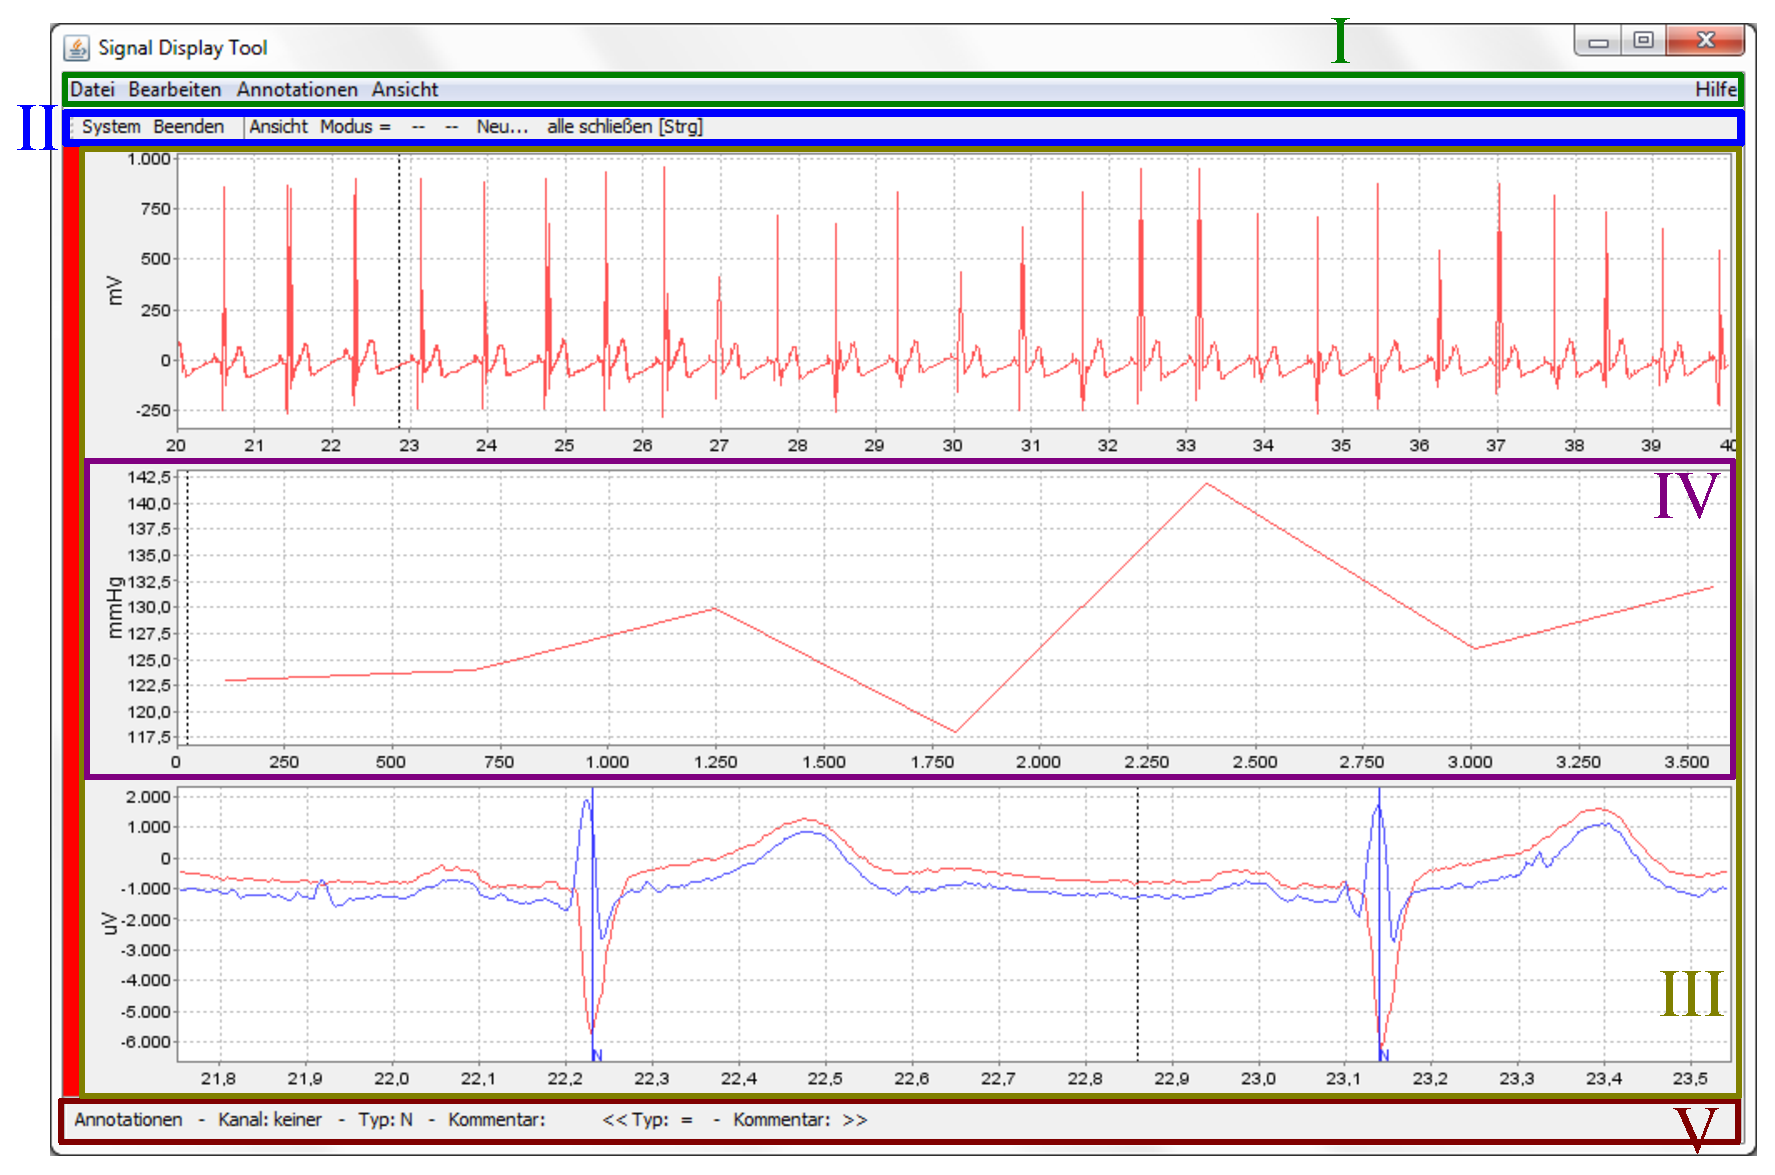
\includegraphics[width=\textwidth]{bilder/programm_ansicht.eps}
\caption[Klassen der grafischen Elemente]{Klassen der grafischen Elemente: I \texttt{Menus}, II \texttt{Toolbar}, III \texttt{SignalPanel}, IV \texttt{SignalView}, V \texttt{StatusBar}}
\label{pic:gui_elements_and_classes}
\end{figure}

\subsection{[WIP]Datenvisualisierung}

- Nutzung von JFreeChart (\ac{lgpl})

\subsection{[WIP]Umsetzung der \ac{GUI} im Paket \class{gst.ui}}

\begin{figure}[htb]
\centering
\includegraphics[angle=-90, width=0.9\textwidth]{bilder/package_ui_ubersicht.pdf}
\caption{"Ubersicht "uber das \class{ui}-Paket}
\label{pic:package_ui_ubersicht}
\end{figure}

- alle Elemente Singleton (bis auf \class{SignalView})

\subsubsection{[WIP]Koordiniertes Zoomen und Scrollen durch \class{SignalPanel}}

- Observer-Prinzip
- zwei eigene Managerklassen (Unabh"angigkeit)

\subsubsection{[WIP]Darstellung und Verarbeitung der Benutzereingaben}

- \class{SignalView} stellt dar
- Datenzugriff "uber abstrakte Definition von \class{DataController}
- Subklassen verarbeiten Maus- und Tastatureingabe

\subsubsection{[WIP]Verarbeitung und Ver"anderung von Annotationen}

- Einf"ugen von Annotationen "uber \class{AnnotationManager}
- Dreiecksbeziehung von \class{Annotation\-Controller}, \class{AnnotationList} und \class{AnnotationManager} erl"autern
- Suchalgorithmus zum finden der aktuellen Annotation
- "Anderung wird durch die Implementierung vom Interface \class{Data\-Change\-Listener} automatisiert aktualisiert



%% EOF %%%%%%%%%%%%%%%%%%%%%%%%%%%%%%%%%%%%%%%%%%%%%%%%%%%%%%
